\documentclass[fleqn,10pt]{physiome}
% Use option lineno for line numbers 
\usepackage{tabularx}

\articletype{Original}
%% Choose from Original, Retrospective, Review, Letter

\title{Mathematical model of excitation-contraction in a uterine smooth muscle cell}

\author[1][weiwei.ai@auckland.ac.nz]{Weiwei Ai}
\author[2]{Limor Freifeld}
\author[1]{David P Nickerson}
\affil[1]{Auckland Bioengineering Institute, University of Auckland, New Zealand}
\affil[2]{Department of Biomedical Engineering, Technion – Israel Institute of Technology, Haifa, Israel}


%% The following lines can be omitted when submitting;
%% information will be added by editors
\publicationdate{28 Oct 2021}
\editor{Shelley Fong}
\curator{Karin Lundengård}
\submitteddate{4 Oct 2021}
\accepteddate{19 Oct 2021}
\citethisas{Ai et al. (2021)\\Mathematical model of excitation-contraction in a uterine smooth muscle cell. Physiome.}{10.36903/physiome.16828756}
\begin{document}

\maketitle

\begin{abstract}
The \citet{bursztyn2007mathematical} paper proposes a mathematical model of excitation-contraction in a myometrial smooth muscle cell (SMC). The model incorporates processes of intracellular $Ca^{2+}$ concentration control, myosin light chain (MLC) phosphorylation and stress production. We create a modularized CellML implementation of the model, which is able to simulate these processes against the original data.
\end{abstract}

\keywords{cellular calcium control mechanisms, myometrial contractions, computational model, CellML}

\primarypubs[10.36903/physiome.16828756]{sample}{bursztyn2007mathematical}

\section{Introduction}
The model \citep{bursztyn2007mathematical} describes how the intracellular $Ca^{2+}$ concentration increases due to membrane depolarization, which leads to an increase in the myosin phosphorylation rate and therefore the generation of muscle contraction. Here, we divide the mathematical model into distinct sub-modules encoded in CellML enabling reuse of the various sub-modules in future studies and models. We also reuse a few previously developed sub-modules at \url{https://models.physiomeproject.org/workspace/6bc}, such as Nernst potential computation and stimulation protocols, to reduce the implementation workload and potentially improve the model quality. We successfully reproduce control of intracellular $Ca_{i}^{2+}$ concentration, MLC phosphorylation, stress production and sensitivity analysis. From the primary paper we extracted data using the Engauge digitizer software \citep{mitchell_markummitchellengauge-digitizer_2020} to compare the current simulation results against those in the primary publication.

\section{Model description}
\label{sed:modelDescription}

\subsection{Primary Publication}
The model \citep{bursztyn2007mathematical} incorporates three $Ca^{2+}$ control mechanisms: voltage-operated $Ca^{2+}$ channels, $Ca^{2+}$ pumps and $Na^{+}$/$Ca^{2+}$ exchangers, which employ the mathematical formulation proposed in \citep{parthimos1999minimal}. The cross-bridge model of \citet{hai1988cross} is used to describe the processes of myosin light chain (MLC) phosphorylation and stress production, which is essentially a deterministic multi-state Markov model (MM) \citep{19961078}. The primary paper \citep{bursztyn2007mathematical} has shown that the model is able to reproduce the results against experimental data obtained in pregnant rats and measurements in human nonpregnant myometrial cells. There is no publicly available code for this model, making it difficult to reuse this work. We therefore present in this article a CellML implementation for researchers to reuse in further developments based on this model.

\subsection{Modularized CellML model}
The modularized CellML implementation is available in the Physiome Model Repository (PMR) at \url{https://models.physiomeproject.org/workspace/6bb} and the documentation can be found in the corresponding exposure at \url{https://models.physiomeproject.org/e/742}. In this manuscript we focus on reproducibility and reusability. The main components of this model and the performed simulation experiments are summarized as follows.

The \emph{J\_Ca component} defines the fluxes of $Ca^{2+}$ ions, including the flux through the L-type voltage dependent $Ca^{2+}$ channels $J_{VOCC}$, the efflux through $Ca^{2+}$ pump $J_{Ca,pump}$, and the flux through the $Na^{+}/Ca^{2+}$ exchangers $J_{Na/Ca}$. The computation of current through the L-type voltage dependent $Ca^{2+}$ channels reuses the imported \emph{ionic current component} ( \url{https://models.physiomeproject.org/workspace/6bc}). 

The \emph{EC\_uSMC component} combines the excitation description \emph{J\_Ca component}, the reversal potential defined in the \emph{Nernst potential component}, and the imported \emph{CB4HM component} ( \url{https://models.physiomeproject.org/workspace/6bc}). The \emph{CB4HM component} defines the four-state cross-bridge model of \citet{hai1988cross}, where the rate constants of MLC phosphorylation $K_1$ and $K_6$ are regulated by the intracellular $Ca_{i}^{2+}$  concentration. Hence, the link between the excitation and contraction is established through the intracellular $Ca^{2+}$ concentration. The component can simulate MLC phosphorylation and stress production process provided various voltage stimuli. 

To test individual processes, we built the \emph{Unit\_uSMC component}, which decouples the connection between the excitation and contraction, thus enabling the use of an arbitrary $[Ca_{i}^{2+}]$ profile to validate the response of phosphorylation and stress development.  

Following best practices, our CellML implementation separates the mathematics from the parameterisation of the model. The mathematical model is imported into a specific parameterised instance in order to perform numerical simulations. The parameterisation would include defining the stimulus protocol to be applied. We have seven sets of simulation experiments and corresponding simulation results to reproduce the corresponding figures in the primary publication: 
\begin{enumerate}[noitemsep] 
\item the \emph{single stimulation experiment} is used to validate the excitation and contraction response to a single voltage pulse with various durations and levels;
\item the \emph{multiple stimulation experiment} is used compare the reaction to the voltage-pulse train with a single pulse;
\item the \emph{voltage ramp experiment} is used to compute the $Ca^{2+}$ channel activation as a function of $V_m$;
\item the \emph{membrane potential simulation experiment} is used to simulate the excitation and contraction response to a recorded human plateau potential;
\item the \emph{$Na_i^{+}$ experiment} is used to evaluate the variation in the flux through the $Na^{+}/Ca^{2+}$ exchangers as a function of $[Na_i^{+}]$;
\item the \emph{$Ca_{i}^{2+}$ experiment 1} is used to simulate the reaction in human nonpregnant myometrium to an increase in $[Ca_{i}^{2+}]$; and 
\item the \emph{$Ca_{i}^{2+}$ experiment 2} is used to simulate the reaction during stretch-induced phasic contraction of human myometrium.
\end{enumerate}

Simulation settings and detailed solver information are encoded in SED-ML documents for execution of the simulation experiments \citep{waltemath_reproducible_2011}. The Python scripts used with OpenCOR Snapshot 2021-05-19 \citep{garny_opencor_2015} to perform simulations and produce the figures in the primary paper are also included in the folder <./Simulation->src>. The name of the simulation and plot scripts indicates the figure number in the primary paper. For example, Fig2\_sim.py is used to generate the simulation data and Fig2\_plot.py reproduces the graph shown in Figure 2 from \citet{bursztyn2007mathematical}.

\section{Model results}
\label{sed:modelResults}
In the presented figures, the dots denote the simulated data extracted from the primary publication, while the solid lines are the simulation results produced by the current CellML implementation.

\subsection{Control of Intracellular $Ca_{i}^{2+}$  Concentration}
To simulate the intracellular $Ca^{2+}$ concentration decay, we need to increase the $[Ca_{i}^{2+}]$ first. In the experimental paper \citep{shmigol1998carboxyeosin}, they used a train of pulses from a holding potential of $-80$~mV to a step potential of $0$~mV to generate an increase in $[Ca_{i}^{2+}]$. In our simulation of Figure 2A, we set the $[Ca_{i}^{2+}]$ value at time $t=0$ to the experimentally measured one, i.e., $980.63$~nM, and simulate the subsequent $Ca_{i}^{2+}$ decay due to extrusion of $Ca_{i}^{2+}$ by the $Na^{+}/Ca^{2+}$ exchangers only. Figure 2B describes a second simulation under similar conditions but with both $Ca_{i}^{2+}$ extrusion mechanisms (exchanges and pumps) active. The membrane potential throughout the simulation holds at $-80$~mV and the corresponding $[Na_{i}]$ is $16.55$~mM.

In the simulation of Figure 3 from the primary paper, the holding voltage is $-50$~mV and the corresponding $[Na_{i}]$ is $2.9836$~mM. At time $t=0$, the initial value of $[Ca_{i}^{2+}]$ is set to $130$~nM, while a $200$-ms pulse voltage is applied. The potential levels vary from plot A to C. Figure 4 uses the similar settings with different pulse potentials as well. 

The experiment setting is summarized in \autoref{tab:clamp} and the simulation results are shown in Figures \ref{simFig2}, \ref{simFig3} and \ref{simFig4}.

\begin{table}[hbt!]\centering
\caption{Experiment setting}\label{tab:clamp}
\begin{tabularx}{\textwidth}{m{1cm}m{3cm}m{3cm}m{2.3cm}XX}
\toprule
Fig & Test voltage (mV) &  Pulse duration (ms) & $[Na_i]$ (mM) & Initial $[Ca_i]$ (nM)\\
\midrule
2A &  NA  & NA & 16.55 & 980.63 \\
2B &  NA & NA & 16.55 & 980.63\\
3A & 0 & 200 & 2.9836 & 130\\
3B & 10 & 200  & 2.9836 & 130\\
3C &  -10 & 200  & 2.9836 & 130\\
4A & -20 & 200  & 2.9836 & 130\\
4B &  20 & 200  & 2.9836 & 130 \\
\bottomrule
\end{tabularx}
\end{table}

\begin{figure}
\centering
\begin{minipage}[t]{\dimexpr.5\textwidth-0.2em}
  \centering
  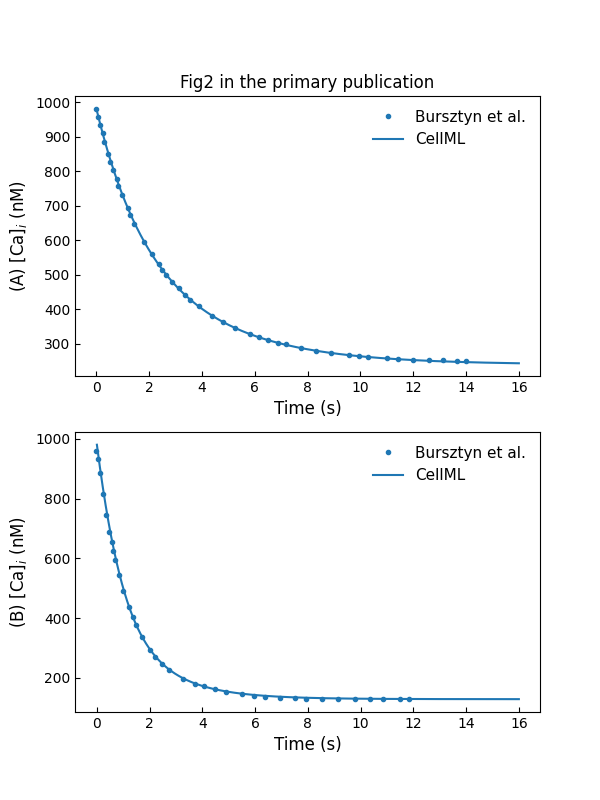
\includegraphics[width=\linewidth]{./figs/simFig2.png}
  \caption{Simulations of $[Ca_{i}^{2+}]$ decay (in nM). A: under inhibition of $Ca^{2+}$ pumps. B: in control conditions (\emph{c.f.,} Fig.~2 in \citet{bursztyn2007mathematical}).}
  \label{simFig2}
\end{minipage}\hfill
\begin{minipage}[t]{\dimexpr.5\textwidth-0.2em}
  \centering
  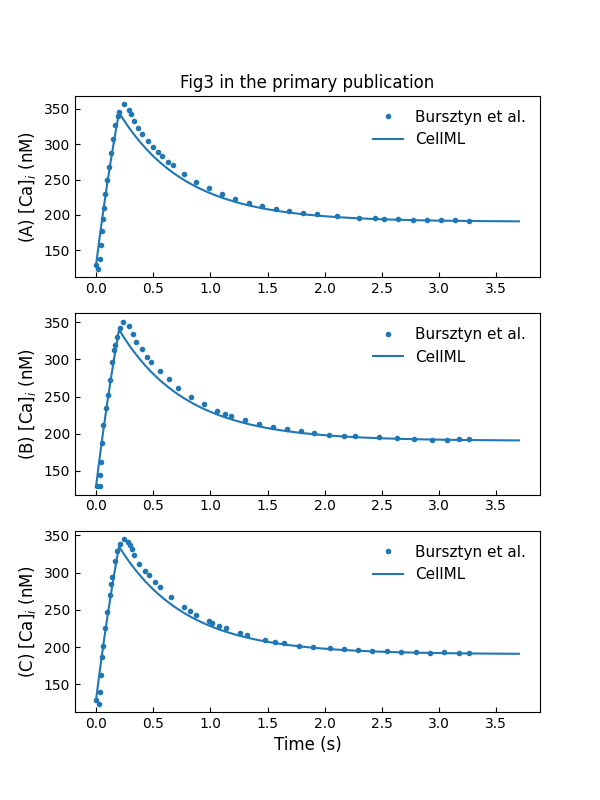
\includegraphics[width=\linewidth]{./figs/simFig3.png}
  \caption{Simulation of $[Ca_{i}^{2+}]$ rise and decay following a $200$-ms voltage pulse of $0$ mV (A), $10$ mV (B), and $-10$ mV (C) (\emph{c.f.,} Fig.~3 in \citet{bursztyn2007mathematical}).}
  \label{simFig3}
\end{minipage}
\end{figure}

The experiment setting to reproduce primary Figure 5A and 5B are the same as the one used in primary Figure 2B and Figure 3A, respectively. The simulation results are shown in \autoref{simFig5}. Plot A shows $Ca^{2+}$ flux through $Na^{+}/Ca^{2+}$ exchangers and $Ca^{2+}$ pumps during $[Ca_{i}^{2+}]$ decay at a holding voltage of $-80$~mV, while plot B shows $Ca^{2+}$ flux through $Ca^{2+}$ channels and $Ca^{2+}$ extraction mechanisms during $[Ca^{2+}]$ rise and decay in response to a $200$-ms voltage pulse to $0$~mV from holding potential of $-50$~mV.

\begin{figure}
\centering
\begin{minipage}[t]{\dimexpr.5\textwidth-0.2em}
  \centering
 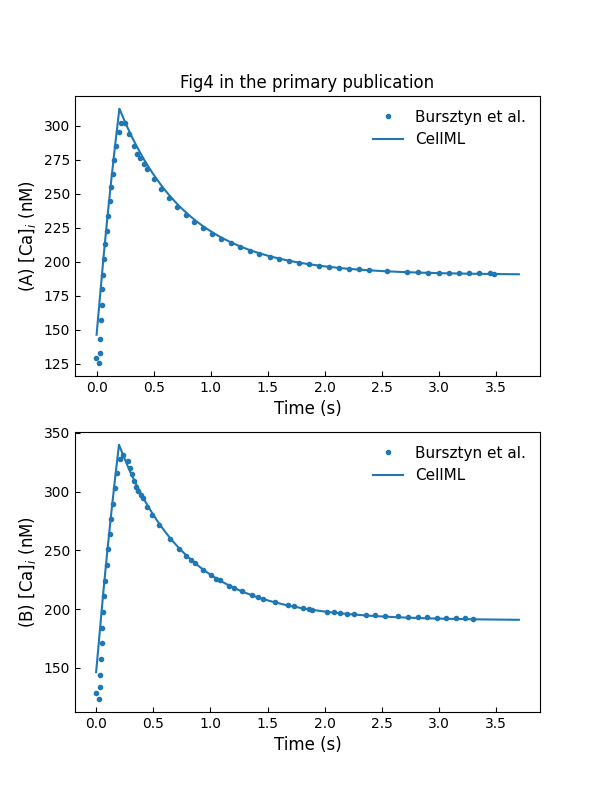
\includegraphics[width=\linewidth]{./figs/simFig4.png}
\caption{Simulation of $[Ca_{i}^{2+}]$ rise and decay following a $200$-ms voltage pulse of $-20$ mV (A), $20$ mV (B) (\emph{c.f.,} Fig.~4 in \citet{bursztyn2007mathematical}).}
\label{simFig4}
\end{minipage}\hfill
\begin{minipage}[t]{\dimexpr.5\textwidth-0.2em}
  \centering
  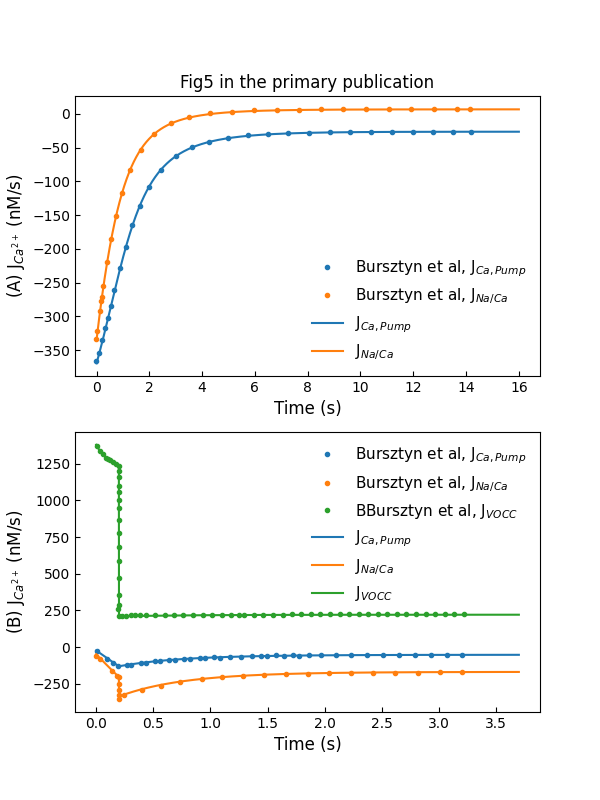
\includegraphics[width=\linewidth]{./figs/simFig5.png}
  \captionof{figure}{Simulations of $Ca^{2+}$ fluxes through various $Ca^{2+}$ control mechanisms, including $Ca^{2+}$ entry and extraction from the cell (\emph{c.f.,} Fig.~5 in \citet{bursztyn2007mathematical}).}
  \label{simFig5}
\end{minipage}
\end{figure}

\autoref{simFig6} shows the model reaction to a train of pulse potentials.

\begin{figure}[ht]\centering
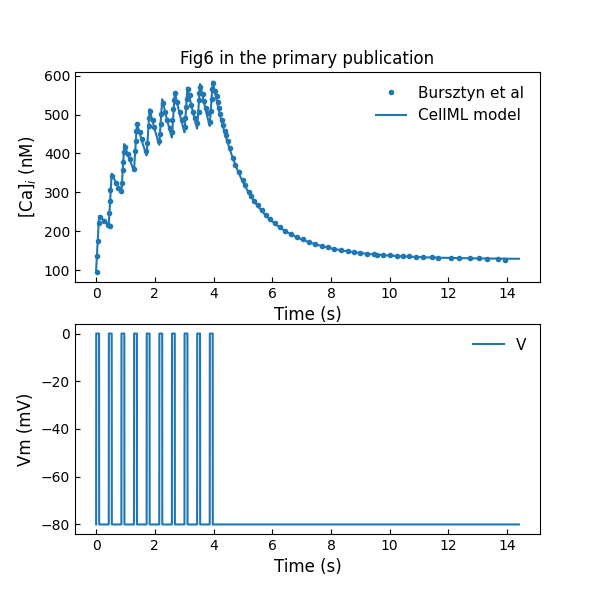
\includegraphics[width=0.7\linewidth]{./figs/simFig6.png}
\caption{Simulation of $[Ca_{i}^{2+}]$ rise and decay in response to a train of 10 voltage pulses of $100$~ms duration from a holding potential of $-80$~mV to a pulse potential of $0$~mV, with an interval of $330$~ms between the pulses (\emph{c.f.,} Fig.~6 in \citet{bursztyn2007mathematical}).}
\label{simFig6}
\end{figure}

\subsection{Sensitivity Analysis}

The effect of parameter $K_{Ca,1/2}$ and intracelluar $Na^{+}$ concentration $[Na_i^+]$ is shown in \autoref{simFig7} and \autoref{simFig8}.  \autoref{simFig7}A and \autoref{simFig8}A simulations are performed on a holding potential of $-50$~mV and the experiment setting is listed in \autoref{tab:clamp2}. We provide a voltage ramp ranging from $-100$~mv to $60$~mV to compute the activation function $\rho_{VCa}$ in \autoref{simFig7}B. While the linear $[Na_i^{+}]$ from $1$~mM to $46$~mM is created to compute the flux $J_{Na/Ca}$ in \autoref{simFig8}B, the membrane potential holds at $-50$~mV. 

\autoref{simFig7}A shows the variation in $[Ca_{i}^{2+}]$ decay following a $200$-ms voltage pulse to $0$ mV due to changes in $K_{Ca,1/2}$, while the variation in the activation function in \autoref{simFig7}B indicates the fractional amount of open VOCCs. 

\autoref{simFig8}A shows the variation in $[Ca_{i}^{2+}]$ rise and decay following a $200$-ms voltage pulse to $0$ mV due to changes in $[Na_i]$, while \autoref{simFig8}B shows the variation in the flux through $Na^{+}/Ca^{2+}$ exchangers.

\begin{table}[hbt!]\centering
\caption{Experiment setting}\label{tab:clamp2}
\begin{tabularx}{\textwidth}{m{1cm}m{2.6cm}m{3cm}m{3cm}X}
\toprule
Fig &  Test voltage (mV) &  Pulse duration (ms)& $[Na_i]$ (mM) & Initial $[Ca_i]$ (nM)\\
\midrule
7A & 0  & 200  & 2.9836 & 130 \\
8A & 0 & 200  & shown in the legend & 130\\
\bottomrule
\end{tabularx}
\end{table}

\begin{figure}
\centering
\begin{minipage}[t]{\dimexpr.5\textwidth-0.3em}
  \centering
 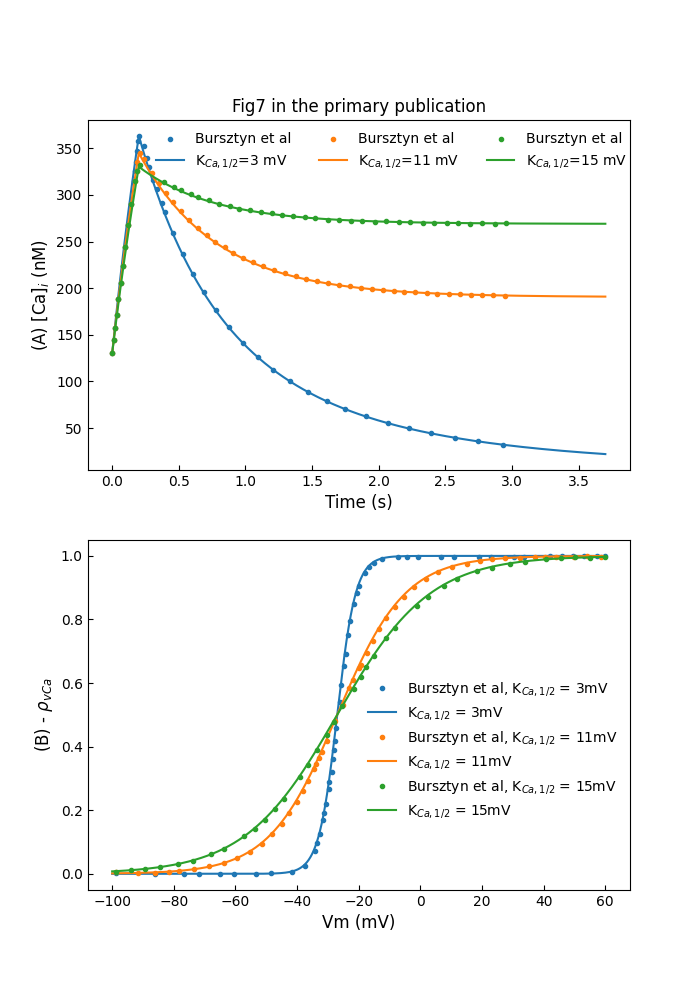
\includegraphics[width=0.9\linewidth]{./figs/simFig7.png}
  \caption{Sensitivity analysis for $K_{Ca,1/2}$. A: variation in $[Ca_{i}^{2+}]$ decay B: variation in the activation function (\emph{c.f.,} Fig.~7 in \citet{bursztyn2007mathematical}).}
  \label{simFig7}
\end{minipage}\hfill
\begin{minipage}[t]{\dimexpr.5\textwidth-0.3em}
  \centering
  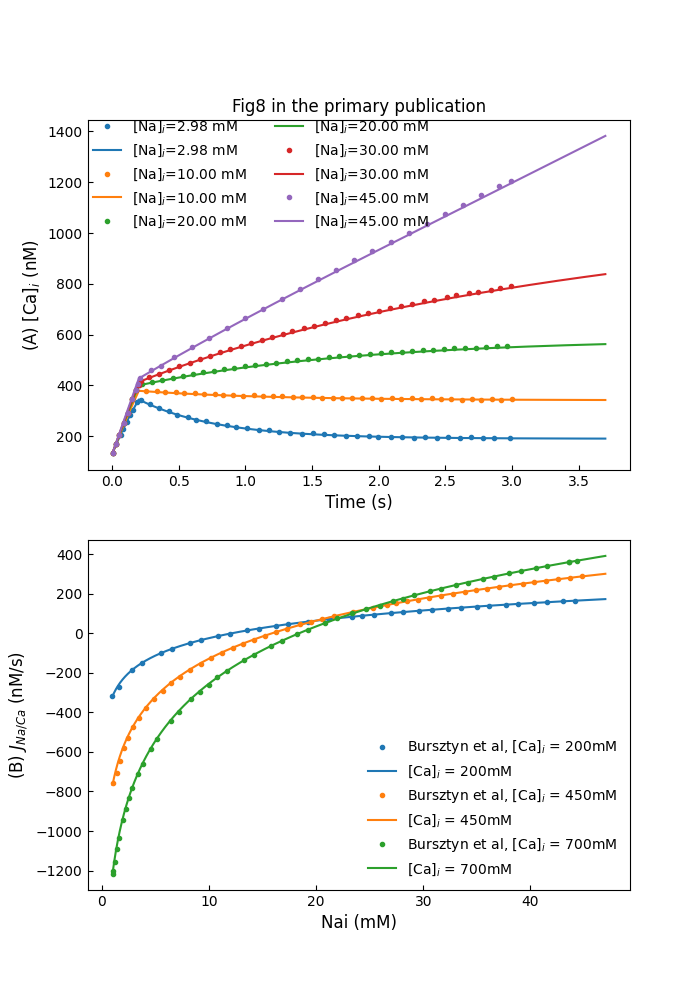
\includegraphics[width=0.9\linewidth]{./figs/simFig8.png}
  \caption{Sensitivity analysis for $[Na_{i}^{+}]$. A: variation in $[Ca_{i}^{2+}]$ rise and decay. B: variation in the flux through $Na^{+}/Ca^{2+}$ exchangers (\emph{c.f.,} Fig.~8 in \citet{bursztyn2007mathematical}).}
  \label{simFig8}
\end{minipage}
\end{figure}

\subsection{MLC Phosphorylation and Stress Production by the Contracting Cell}
We use a curve fitting method to generate a $[Ca_{i}^{2+}]$ profile close to the measured values. This $[Ca_{i}^{2+}]$ is used to drive the cross-bridge model of \citet{hai1988cross}. The simulation result is shown in \autoref{simFig9}. To simulate the stretch-induced contraction and relaxation, we use a piecewise linear function to construct the input $[Ca_{i}^{2+}]$. The model response to the piecewise linear function is shown in \autoref{simFig10}.

\begin{figure}
\centering
\begin{minipage}[t]{\dimexpr.5\textwidth-0.2em}
  \centering
 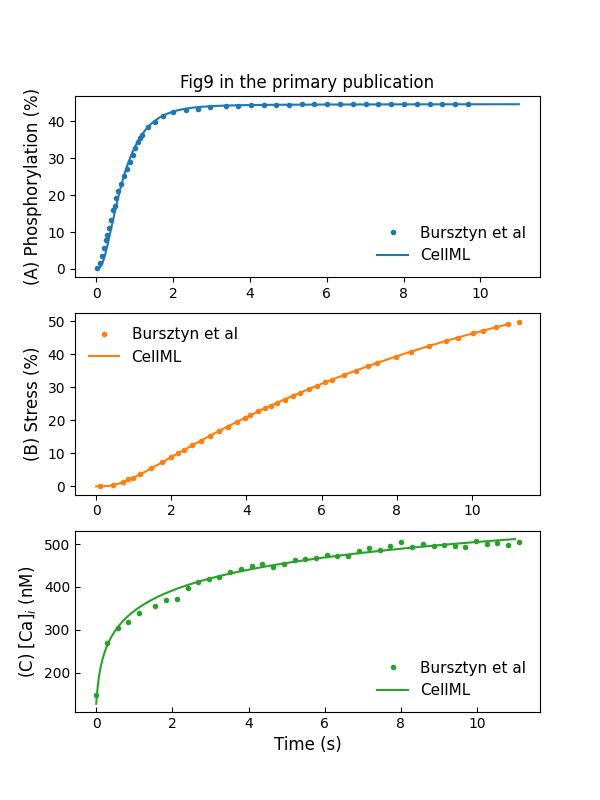
\includegraphics[width=0.9\linewidth]{./figs/simFig9.png}
  \caption{Simulation of MLC phosphorylation (A) and force production (B) stress in response to an increase in $[Ca_{i}^{2+}]$ (C) (\emph{c.f.,} Fig.~9 in \citet{bursztyn2007mathematical}).}
  \label{simFig9}
\end{minipage}\hfill
\begin{minipage}[t]{\dimexpr.5\textwidth-0.2em}
  \centering
  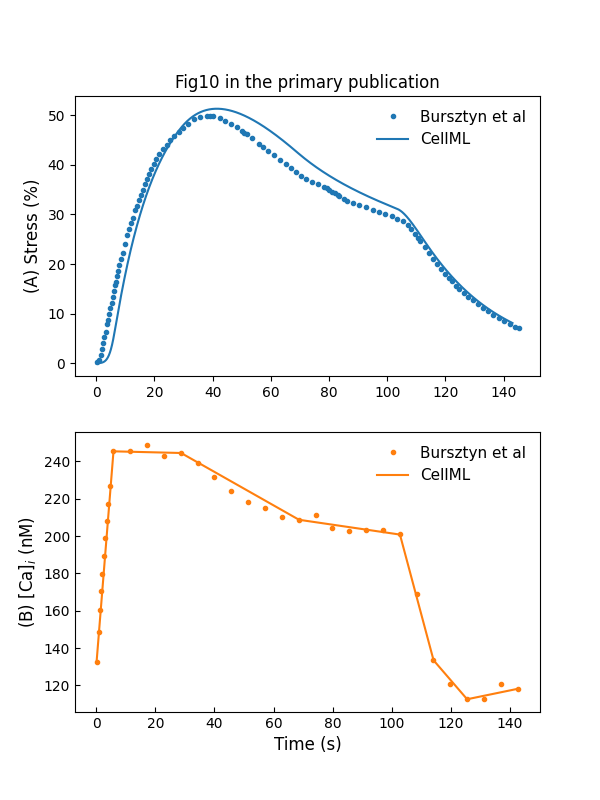
\includegraphics[width=0.9\linewidth]{./figs/simFig10.png}
  \caption{Stress development and relaxation during stretch-induced phasic contraction of human myometrium (\emph{c.f.,} Fig.~10 in \citet{bursztyn2007mathematical}).}
  \label{simFig10}
\end{minipage}
\end{figure}


\subsection{Simulation of $Ca^{2+}$ Control and Stress Production}
The whole model simulation is performed by providing pacing voltage pulses mimicking the membrane depolarization. \autoref{simFig11}A shows the response to a single 1-s voltage pulse from a holding potential of $-80$ mV to a pulse potential of $0$ mV, while \autoref{simFig11}A shows the response to a train of 10 pulses from a holding potential of $-80$ mV to a pulse potential of $0$ mV, which has a duration of $100$ ms and the interval between pulses is $330$ ms.

We use a piecewise linear function to simulate a recorded human plateau potential of pregnant myometrium. \autoref{simFig12} shows the reaction of the cell model to this action potential following a holding potential of $-50$ mV.

The experiment setting for \autoref{simFig11} and \autoref{simFig12} is summarized in \autoref{tab:clamp3}

\begin{table}[hbt!]\centering
\caption{Experiment setting}\label{tab:clamp3}
\begin{tabularx}{\textwidth}{m{1cm}m{7.2cm}m{2cm}X}
\toprule
Fig &  Test Pulse& $[Na_i]$ (mM) & Initial $[Ca_i]$ (nM)\\
\midrule
11A & single 1-s pulse of 0 mV & 16.55 & 130 \\
11B & ten 100-ms pulses of 0 mV with 300-ms interval & 16.55 & 130\\
12 & simulated action potential & 2.9836 & 39\\
\bottomrule
\end{tabularx}
\end{table}

\begin{figure}
\centering
\begin{minipage}[t]{\dimexpr.5\textwidth-0.2em}
  \centering
 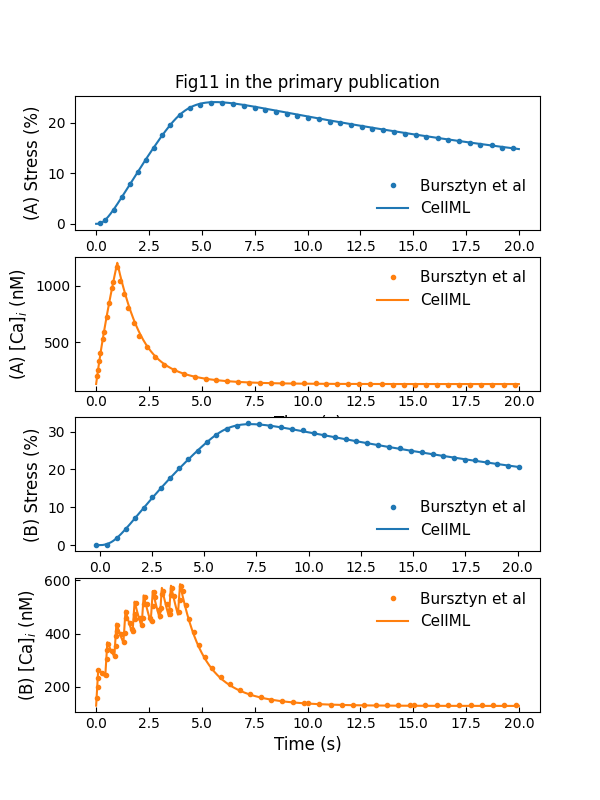
\includegraphics[width=\linewidth]{./figs/simFig11.png}
  \captionof{figure}{Simulations of changes in $[Ca_{i}^{2+}]$ and stress in response to pacing pulses (\emph{c.f.,} Fig.~11 in \citet{bursztyn2007mathematical}).}
  \label{simFig11}
\end{minipage}\hfill
\begin{minipage}[t]{\dimexpr.5\textwidth-0.2em}
  \centering
  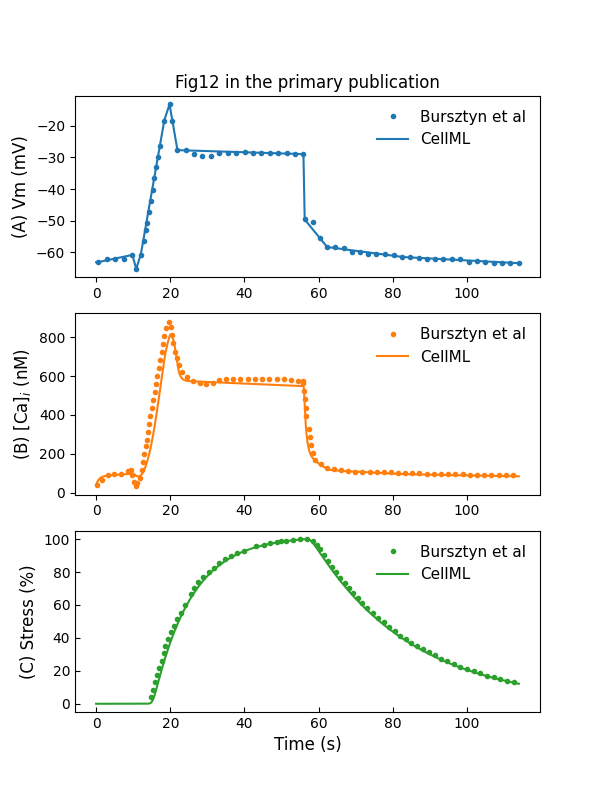
\includegraphics[width=\linewidth]{./figs/simFig12.png}
  \captionof{figure}{Simulation of changes in $[Ca_{i}^{2+}]$ and stress in response to a plateau potential $V_m$ (\emph{c.f.,} Fig.~12 in \citet{bursztyn2007mathematical}).}
  \label{simFig12}
\end{minipage}
\end{figure}

\section{Discussion}
\label{sec:discussion}
We implemented the model \citep{bursztyn2007mathematical} using CellML in a modularized style which can be reused in future. We have successfully replicated all the figures and summarized detailed experiment settings for simulation in \autoref{sed:modelResults}. 
In doing this, we noticed trivial typographical errors in parameter units and references in Table~$3$ of \cite{bursztyn2007mathematical}. Hence, we correct these in \autoref{tab:parameters} to remove potential confusion.

\begin{table}[h!]\centering

\caption{Correction of primary Table 3}\label{tab:parameters}

\begin{tabular}{lccrr}
\toprule
Parameters & primary paper & current CellML\\
\midrule
$V_{p,max}$ & 5.1449e-4 $mM\cdot s^{-1} \cdot mV^{-1}$  & 5.1449e-4 $mM\cdot s^{-1} $ \\
$G_{Na/Ca}$ & 5.7297e-5 $mM\cdot s^{-1} \cdot mV$  & 5.7297e-5 $mM\cdot s^{-1} \cdot mV^{-1}$ \\
$[Na_{i}]$ & 16.55 $mM$ (18) & 2.9836 $mM$ (18)\\
$[Na_{i}]$ & 2.9836 $mM$ (19) & 16.55 $mM$ (19)\\
\bottomrule
\end{tabular}
\end{table}

Another implementation note is that the primary paper used ``efflux'' to indicate the direction of $J_{ca,pump}$ described in Equation (4) with a positive sign. In CellML implementation, the direction information is included in the equation. That is, 
\begin{equation}
    J_{Ca,pump}(t)=-V_{pmax}\dfrac{[Cai(t)]^n}{[K_{ph}]^n+[Cai(t)]^n}
\end{equation}
Consequently, CellML model uses a positive sign before the term $J_{ca,pump}$ in the intracellular calcium concentration equation:
\begin{equation}
    \frac{\mathrm{d}Cai(t) }{\mathrm{d} t}=J_{VOCC}(t)+J_{Ca,pump}(t)+J_{Na/Ca}(t)
\end{equation}

\section{Acknowledgement}
The Freifeld lab is supported by the Zuckerman STEM Leadership Program and the Taub family foundation.

\bibliography{sample}

\end{document}